\subsection*{Surface enrichment of betaine uptake and peroxide defence accompanies community turnover}

To test whether the compartment differences observed in the amplicon survey extend to encoded metabolic and stress-response capacities, we first compared ecological contrasts inferred from PICRUSt2 with those derived from the 5,438 species-representative genomes (\texttt{EQ-MAG-\allowbreak REFINED-\allowbreak v1.0.0}) in the 442 exact specimen-matched libraries (\texttt{EQ-COVERM-\allowbreak REL-\allowbreak ABUND-\allowbreak v1.0.0}). Across 8,860 shared KOs normalised to each platform's complete KO total, surface--subsurface and root-adjacent--subsurface effect sizes were moderately correlated between methods (Spearman $\rho=0.52$, 95\% spatial-block CI $0.31$--$0.54$, and $\rho=0.55$, 95\% CI $0.43$--$0.57$, respectively), and their directions agreed for $67.0\%$ and $67.8\%$ of KOs (Supplementary Section~\ref{si-sup:mag_integration}). Because marker-gene prediction captured only part of the genome-resolved functional variation between soil compartments, we evaluated selected functional groups and their carriers directly in the shotgun metagenomes and recovered genomes.

We evaluated 41 published microTrait rules \cite{karaoz2022microtrait} using protein-profile searches on the 20,451,986 representative-genome proteins called by Pyrodigal (\texttt{EQ-PROT-\allowbreak PYRODIGAL-\allowbreak REP-\allowbreak v1.0.0}) and separately projected the rules onto the frozen analytical representative-genome KO matrix (\texttt{rep\_ko\_v2.tsv}; Methods and Supplementary Section~\ref{si-sup:mag_integration}). The panel distinguished compatible-solute uptake from de novo synthesis and acute exposure protection from baseline DNA maintenance. In paired comparisons across 68 visits at 36 sites, the mapped community had greater representation of the BetL glycine-betaine transporter (K02168) and the AhpCF peroxide-reduction system (K03386/K03387) at the surface than in shallow subsurface soil (Figure~\ref{fig:mag_functions}a). The mean surface excess was $7.6$ and $6.9$ percentage points, respectively. Both contrasts retained positive spatial-block intervals under the KO projection, with the original-read denominator, in higher-quality genomes ($\ge 70\%$ completeness, $\le 5\%$ contamination) and in the 442-library matched amplicon cohort across 58 sites. Spatial models across the 545 read-depth-annotated metagenomes adjusting for campaign, read depth and dune field supported the same directions ($+6.70$ percentage points, 95\% CrI $5.24$--$8.16$ for BetL; $+5.53$ percentage points, 95\% CrI $3.84$--$7.22$ for AhpCF; Supplementary Table~\ref{si-tab:mag_spatial}).

The full microTrait workflow on all 5,438 genomes retained these surface associations under a separate gene-calling and rule-processing implementation (\texttt{EQ-MICROTRAIT-\allowbreak REP-\allowbreak v1.0.0}; \cite{rubalkhali_datapaper}). In the same 68 paired visits, the estimated surface excess was about 6.9 percentage points for each trait, with positive spatial-bootstrap intervals under both mapped-community and original-read denominators (Supplementary Table~\ref{si-tab:microtrait_sensitivity}). The BetL contrast was slightly smaller than in the initial profile screen, whereas the AhpCF contrast changed little.

The broader 41-rule trait panel distinguished these associations from a uniform increase in stress-response genes. Surface communities also had greater representation of photolyase and carotenoid markers, whereas superoxide dismutase and betaine-biosynthesis contrasts remained uncertain. DNA-repair markers differed in their responses: mismatch repair was enriched at the surface, while base-excision repair showed little difference. Trehalose results depended on the annotation rule. The complete panel, including uncertain and annotation-sensitive results, is reported in Supplementary Table~\ref{si-tab:stage4_selected_panel}.

Using GTDB release 232 assignments, changes in community membership accounted for most of these contrasts: between-genus replacement contributed $5.9$ percentage points to the BetL difference and $5.3$ points to the AhpCF difference, changes within shared genera contributed less than $0.3$ percentage points in either direction, and the remainder came from groups detected in only one compartment (Supplementary Table~\ref{si-tab:canonical_turnover_3guilds}); the earlier taxonomy snapshot gave a similar decomposition (Figure~\ref{fig:mag_functions}b). Supplementary Section~\ref{si-sup:mag_integration} reports annotation-sensitive results, taxonomy-snapshot provenance and the treatment of genomes without genus assignments.

Genome-resolved profiles also identified archaeal populations beyond the bacterial focus of the amplicon survey, with Thermoplasmatota consistently more represented in shallow subsurface than in surface soil across paired sites (Supplementary Section~\ref{si-sup:mag_integration}). Detailed analyses of archaeal occurrence across the transect and the sequence-dark, export-enriched accessory proteome of these desert Thermoplasmatota are reported in the companion proteome study \cite{proteome_companion}.

\begin{figure}[!htbp]\centering
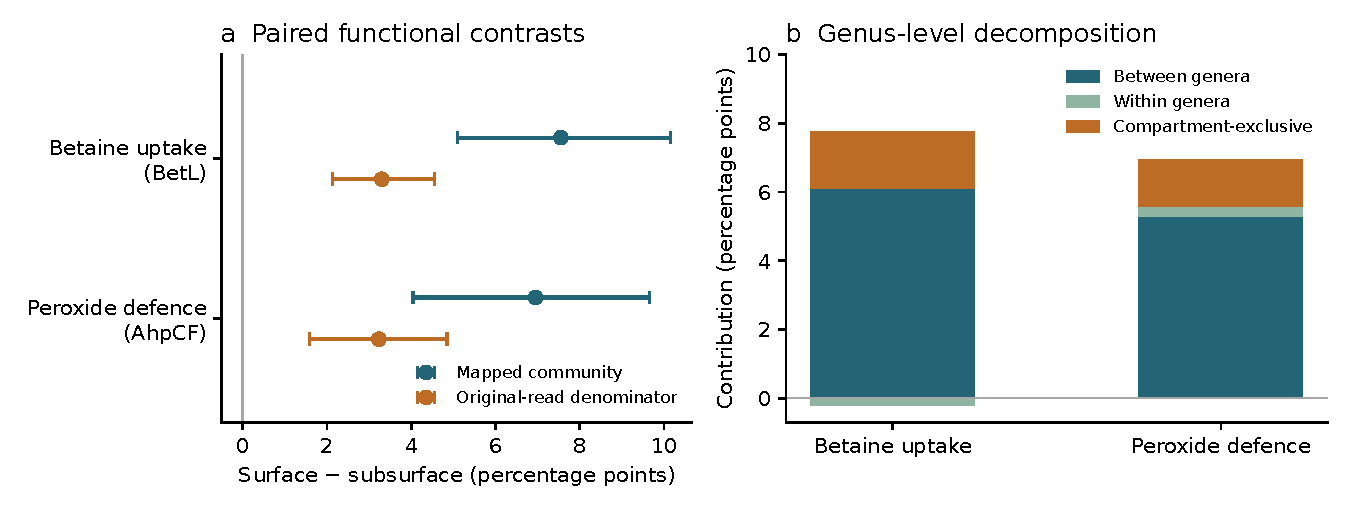
\includegraphics[width=\linewidth]{figures/functional_integration.pdf}
\caption{Surface-associated betaine uptake and peroxide defence accompany community turnover. (a) Mean surface-minus-subsurface differences across 36 sites contributing 68 paired visits. Intervals resample ten contiguous spatial blocks. Gene-content calls use the published BetL and AhpCF profile rules. (b) Exact decomposition into changes between shared genera, changes within those genera and compartment-exclusive contributions under the earlier taxonomy snapshot; the GTDB release 232 decomposition gives the same conclusion (Supplementary Table~\ref{si-tab:canonical_turnover_3guilds}). Replicates are averaged within visits and visit differences within sites. Unclassified genera enter as individual genomes.}
\label{fig:mag_functions}
\end{figure}

\subsection*{Root-adjacent communities have selectively reduced group 1l hydrogen-scavenging capacity}

Oxidation of atmospheric $\mathrm{H}_2$ and $\mathrm{CO}$ by high-affinity hydrogenases and carbon monoxide dehydrogenases is an established energy-conservation strategy supporting microbial persistence in desert soils \cite{ji2017atmospheric,cordero2019atmospheric,bay2021trace,bay2021aridity}. To test whether the distinct root-adjacent communities alter the representation of trace-gas-scavenging guilds across the Rub' al-Khali, we classified hydrogenase and carbon monoxide dehydrogenase large subunits by enzyme group, then quantified their representation directly in metagenomic reads relative to single-copy ribosomal genes. Across 106 depth-matched visits at 47 sites, group 1l $[\mathrm{NiFe}]$-hydrogenase (\texttt{HhyL}) representation was $4.8$-fold lower beside roots than in bulk subsurface soil (median $0.056$ versus $0.271$ genome equivalents; Figure~\ref{fig:loa_guilds}a). Its depletion exceeded the mean change in control hydrogenase and CoxL groups by $1.8$ log$_2$ units (95\% site-bootstrap interval, $1.0$--$2.6$ units of additional depletion; Figure~\ref{fig:loa_guilds}c). This excess persisted across campaigns, sequence-identity thresholds and contamination exclusions. Held-out sequence and simulated-community benchmarks supported recovery of the root-to-bulk contrast (Supplementary Section~\ref{si-sup:loa_methods}).

The spatial model across the 545 read-depth-annotated metagenomes retained the group 1l excess after accounting for campaign, read depth and dune field ($-1.733$ log$_2$ units, 95\% CrI $-2.038$ to $-1.424$; Supplementary Table~\ref{si-tab:mag_spatial}). Root-adjacent contrasts for groups 1h ($-0.083$ log$_2$ units, 95\% CrI $-0.213$ to $0.047$) and 2a ($0.052$ log$_2$ units, 95\% CrI $-0.083$ to $0.187$) were centred near zero. Form-I CoxL showed a small decrease in the spatial model ($-0.117$ log$_2$ units, 95\% CrI $-0.224$ to $-0.011$), whereas its paired contrast was uncertain (raw excess $+0.016$; Supplementary Section~\ref{si-sup:loa}). Group 1l therefore showed the strongest selective root-adjacent depletion. Surface soil had a broader reduction across all four high-affinity groups relative to the controls (Figure~\ref{fig:loa_guilds}b), distinguishing the surface and root-associated patterns.

This functional difference was primarily associated with lineage replacement. Across the 5,438-genome catalogue, the mean root-adjacent change in the mapped share of group 1l carriers was $-18.8$ percentage points: under GTDB release 232 assignments, changes between shared genera ($-11.6$ percentage points) and contributions from compartment-exclusive groups ($-6.8$ percentage points) accounted for almost all of this decrease, whereas the within-genus component was $-0.4$ percentage points, and the earlier taxonomy snapshot gave a similar decomposition (Supplementary Table~\ref{si-tab:canonical_turnover_3guilds}). In an exploratory analysis under the earlier taxonomy snapshot, genus carriage of group 1l remained associated with depletion beside roots after adjustment for predicted maximal growth potential (\texttt{gRodon2} \cite{weissman2021grodon}) and taxonomic order ($p \le 7.4\times 10^{-4}$; [PENDING: \texttt{TAXONOMY-\allowbreak SNAPSHOT-\allowbreak SENSITIVITY}; confirm order- and genus-adjusted \texttt{gRodon2} regression using canonical assignments]). Group 1l representation also declined as extract DNA concentration increased, including within visits and within bulk soil alone. Because extract DNA concentration combines microbial DNA, co-extracted plant DNA and extraction efficiency rather than measuring microbial biomass directly, and metagenomic marker representation measures encoded genetic capacity rather than in situ gas oxidation, this association describes relative guild representation along a DNA-yield gradient (Supplementary Figure~\ref{si-fig:loa_scaling}).

\begin{figure}[!htbp]\centering
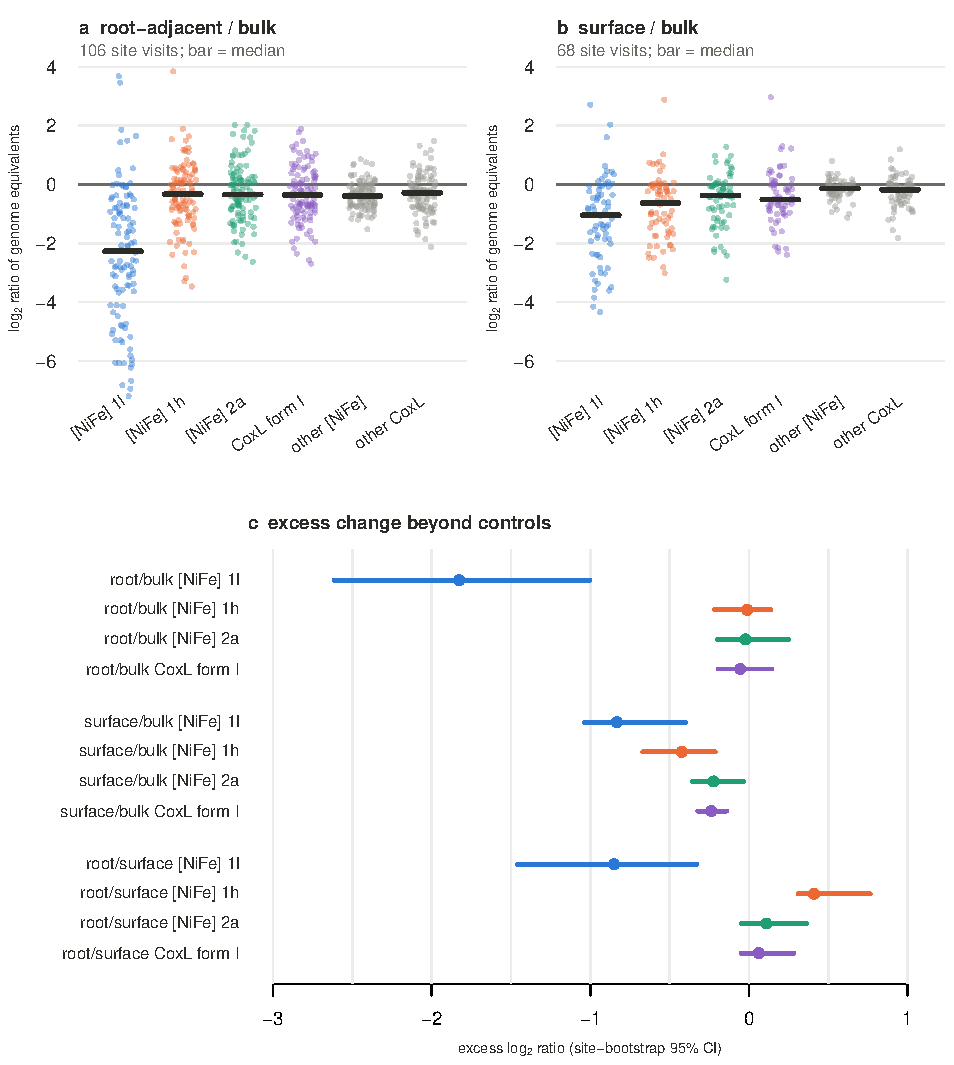
\includegraphics[width=\linewidth]{figures/loa_guilds.pdf}
\caption{Group 1l hydrogenase genes show strong selective depletion beside roots. (a) Log$_2$ ratios of estimated genome equivalents between root-adjacent and bulk subsurface soil at 5--10~cm, for 106 paired visits at 47 sites. (b) Surface versus subsurface soil, for 68 visits at 36 sites. Points are visits and bars are medians. (c) Excess log$_2$ ratios beyond the mean of the two control marker sets, with 95\% site-bootstrap intervals. These paired estimates are complemented by the spatial models in Supplementary Table~\ref{si-tab:mag_spatial}.}
\label{fig:loa_guilds}
\end{figure}
